\chapter{Connaissances biologiques} 

\lettrine{O}{n} s'intéresse dans ce chapitre aux manguiers et aux cécidomyies des fleurs.
On s'intéresse en particulier à leurs descriptions d'un point de vue biologique, leurs développements et leurs intéractions.
Autrement dit, on recence ici les connaissances biologiques nécessaires à la compréhension de notre sujet.


\section{Les manguiers}

Le manguier est un arbre qui a une croissance végétative rythmique.
Cela signifie que sa croissance est entrecoupée par des périodes de repos.
Durant les périodes de croissance, les branches sont prolongées par des tiges qui ont des feuilles.
Ces tiges sont appelées \emph{unités de croissance}. 
Si une unité de croissance prolonge la branche dans l'axe, alors elle est dite apicale ; si elle la prolonge sur le côté, elle sera qualifiée de latérale.
Au fil du temps, les unités de croissance perdent leurs feuilles, durcissent et grossissent jusqu'à faire partie intégrante de la branche.
On peut alors voir le manguier comme un empilement d'unités de croissance;
la base du tronc étant l'unité de croissance la plus ancienne et celles qui portent des feuilles les plus récentes \citep{normand2009}.
Des unités de croissance sont visibles sur la figure~\ref{fig:uc}.
\begin{figure}[ht]
 \centering
 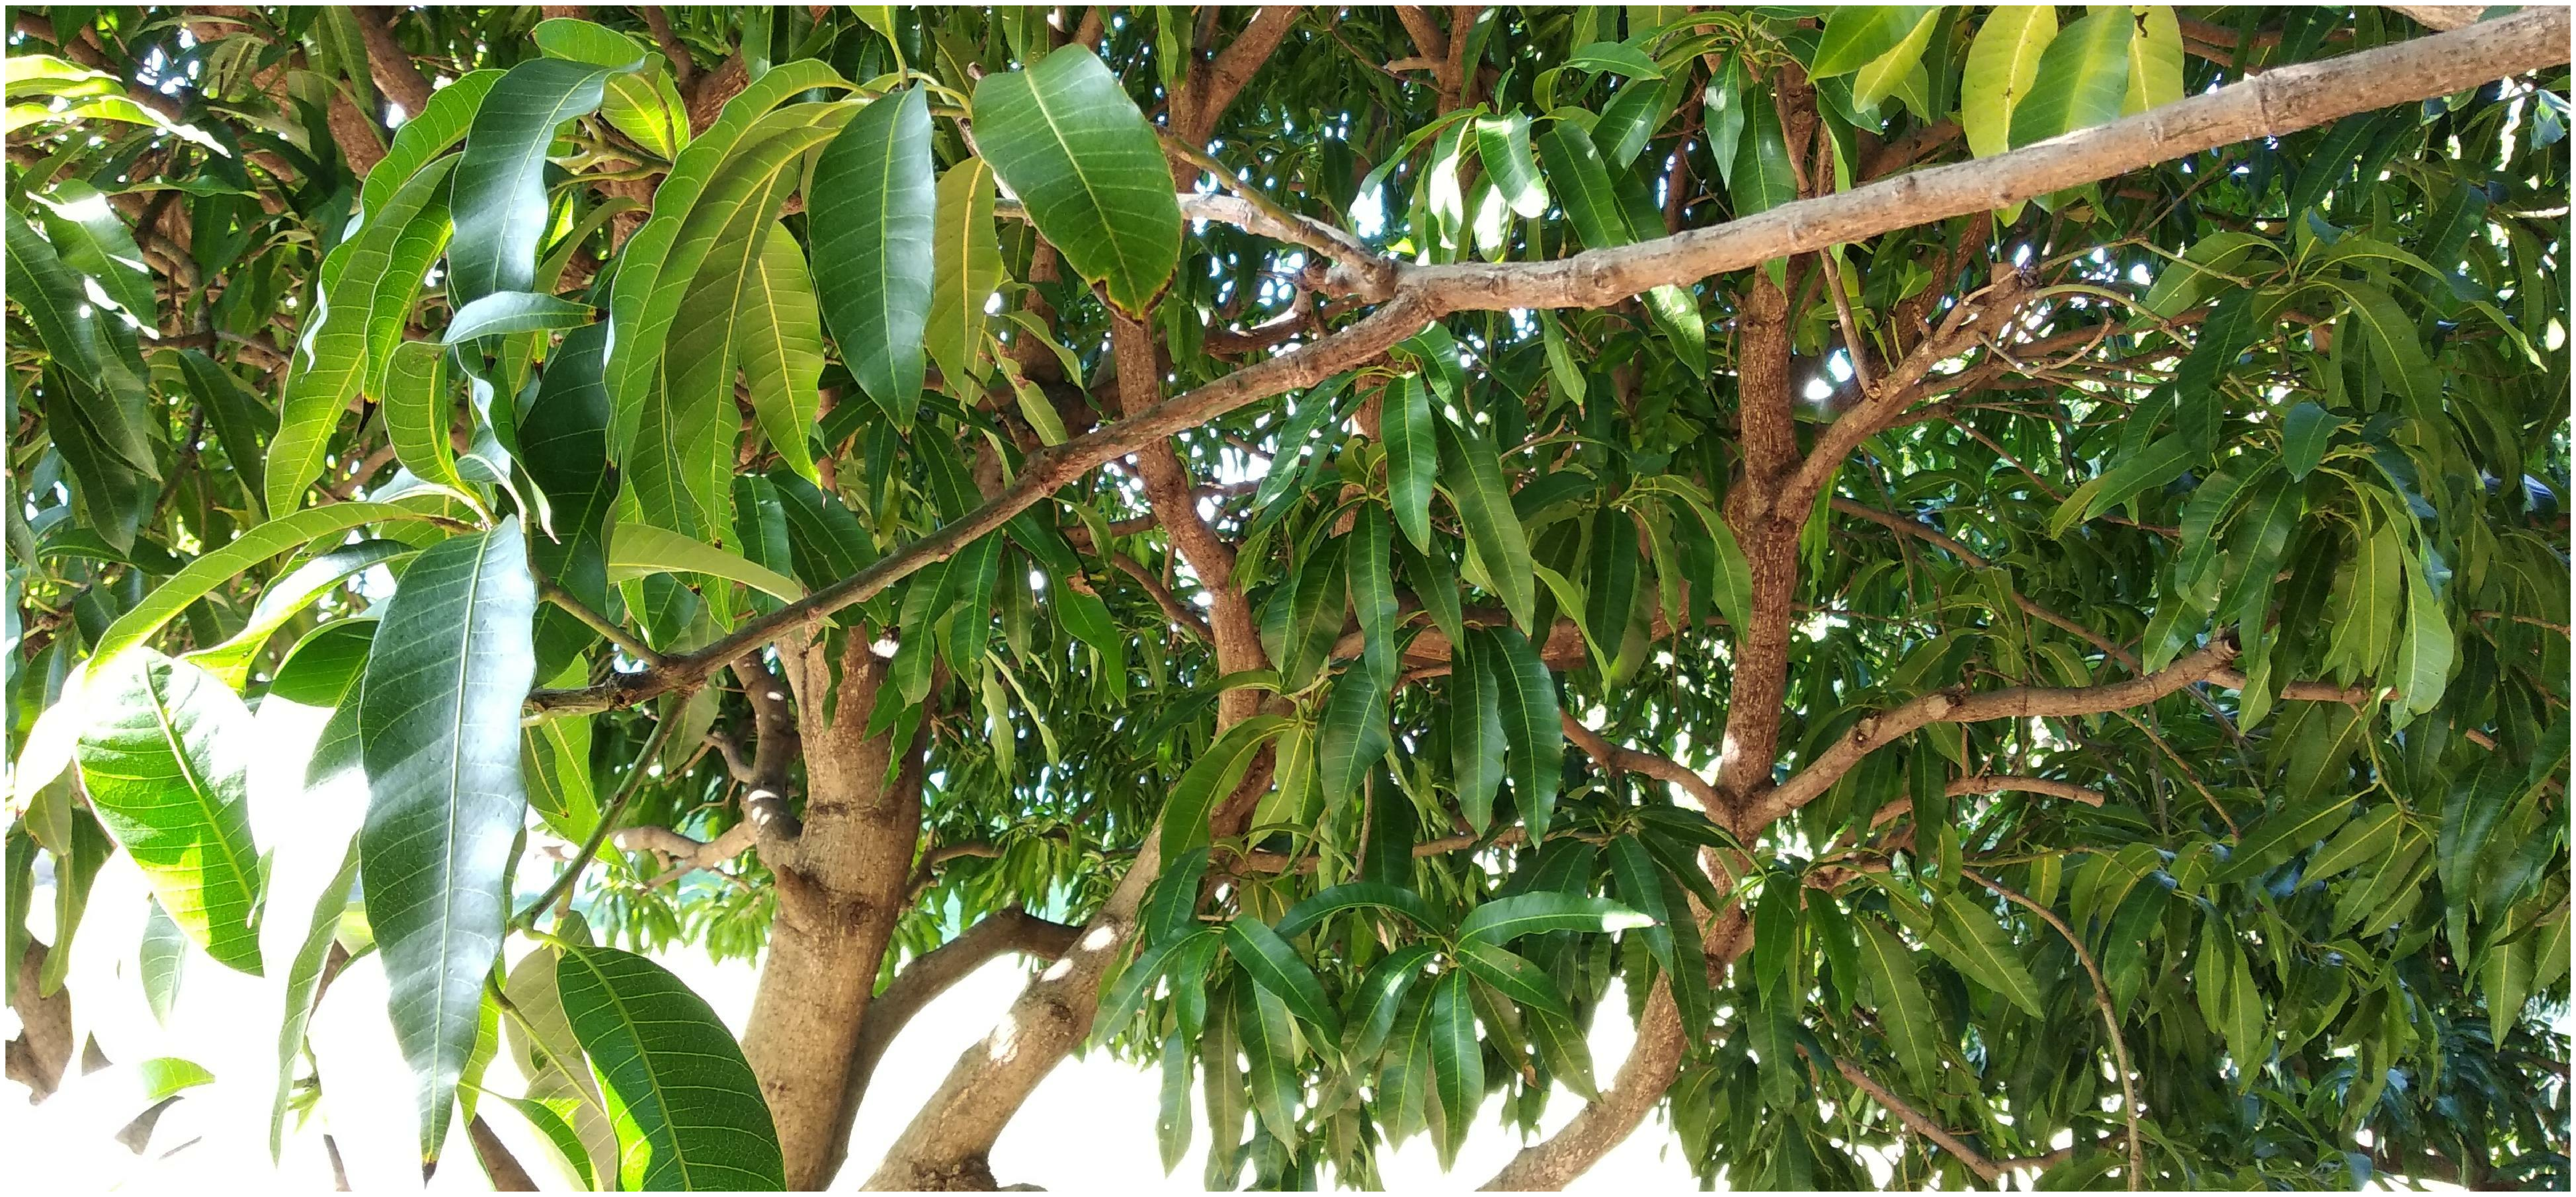
\epsfig{file = photos/uc.eps, scale = 0.09}
 \caption{Photographie d'une branche portant des unités de croissance.}
 \label{fig:uc}
\end{figure}

Et ce sont ces unités de croissance qui portent les \emph{inflorescences}.
Les inflorescences désignent des groupements de bourgeons. 
Ces bourgeons deviennent des fleurs qui elles-même deviennent des fruits, si elles sont fécondées.
En théorie.
En pratique, les bourgeons ne survivent que rarement jusqu'au stade de fruit, ils meurent bien souvent avant.
S'ils meurent parfois à cause des conditions climatiques, la principale raison de leurs morts restent les attaques des ravageurs.

La forte présence des ravageurs s'explique en grande partie par le \emph{cycle phénologique} du manguier.
On désigne par cycle phénologique les phénomènes périodiques qui rythment le monde vivant en fonction des variations climatiques.
Et il y a chez le manguier, en sus des conditions climatiques, d'autres facteurs qui influent sur la phénologie tels que la position de l'unité de croissance ou la charge en fruit de l'année précédente \citep{magne2004effet, normand2009axis}.
Il en résulte que le cycle phénologique est très variable d'un manguier à l'autre.
On observe même des différences au niveau phénologique entre les différentes unités de croissance d'un même arbre.
Mais cela implique aussi que le cycle phénologique peut être modifié (dans une certaine mesure) grâce à des opérations techniques, comme la taille par exemple.

Du cycle phénologique viennent les \emph{stades phénologiques} des inflorescences.
Ils caractérisent le niveau de développement des inflorescences.
On considère ici les stades phénologiques allant de C à F.
Le stade C correspond au débourrement (l'éclosion des bourgeons) de l'inflorescence.
Le stade F s'étend entre l'apparition de la première fleur jusqu'à la disparition de la dernière.
Et les stades D et E représentent les étapes intermédiaires du développement qui mènent du débourrement à la floraison.
Les durées des stades phénologiques sont les suivantes :
\begin{center}
\begin{tabular}{llll}
Stade phénologique & C/D & E & F\\
Durée (en jours) & 7 & 9 & 34
\end{tabular}
\end{center}
Les inflorescences ont ainsi une durée de vie théorique de 50 jours \citep{laurie}. Cette durée théorique peut être réduite en cas d'attaque de cécidomyies des fleurs, surtout lorsque l'inflorescence se fait attaquer lors des premiers stades, moment où l'inflorescence est la plus vulnérable.

La saison des mangues a lieu pendant l'hiver (austral).







\section{Les cécidomyies des fleurs}
